\subsubsection*{Figures and tables for section~\ref{sec:exp3}}
\begin{table}[H]
\caption{Hyperparameters for LOST algorithm.}
\label{tab:LOSTalgo}
\begin{center}
\resizebox{30em}{!}{%
\begin{tabular}{lll}
\toprule
\textbf{Hyperparameter} & \textbf{Value} & \textbf{Source} \\
\midrule
Gram matrix bias b (DINOv2) &
  0.0 &
  Paper, $\S.3.3$ \\
Gram matrix bias b (OpenCLIP) &
  0.1 &
  Paper, $\S.3.3$ \\
Gram matrix bias b (DeiT-III) &
  0.1 &
  Paper, $\S.3.3$ \\
Adjacency threshold $\tau$ &
  0.0 &
  Paper, $\S.3.3$ \\
Feature type (DINOv2) &
  Keys($K$) &
  Paper, $\S.3.3$ \\
Feature type (OpenCLIP, DeiT-III) &
  Values($V$) &
  Paper, $\S.3.3$ \\
Per-row mean-centering of Gram matrix &
  &
  Implementation necessity (see note) \\
Batch size (Table 3 evaluation) &
  32 &
  Implementation choice \\
Workers (Table 3 dataloader) &
  4 &
  Implementation choice \\
\bottomrule
\end{tabular}
}
\end{center}
\end{table}

\begin{table}[H]
\caption{Hyperparameters for linear probing.}
\label{tab:linearprobe}
\begin{center}
\resizebox{35em}{!}{%
\begin{tabular}{lll}
\toprule
\textbf{Hyperparameter} & \textbf{Value} & \textbf{Source} \\
\midrule
Classifier &
  Logistic Regression (\texttt{sklearn}) &
  Paper, $Appendix\ D.2$ \\
Regularisation C &
  1.0 (classification), 0.1 (position) &
  Standard default \\
Max iterations &
  1000 (classification), 300 (position) &
  Convergence heuristic \\
Solver &
  lbfgs &
  Efficient for dense features \\
Feature normalisation &
  \texttt{StandardScaler} (zero mean, unit variance) &
  Standard practice \\
Reconstruction regressor &
  Ridge Regression, $\alpha=1.0$ &
  Standard practice \\
\bottomrule
\end{tabular}
}
\end{center}
\end{table}

\begin{table}[H]
\caption{Hyperparameters for attention map averaging.}
\label{tab:attmapavg}
\begin{center}
\resizebox{\textwidth}{!}{%
\begin{tabular}{lll}
\toprule
\textbf{Hyperparameter} & \textbf{Value} & \textbf{Source} \\
\midrule
\# of images averaged &
  500 &
  Our choice (paper: ``random subset``) \\
Patch token used &
  Centre patch at grid position (18,18) &
  Our choice (all patches show the same qualitative behavior) \\
\texttt{fused\_attn} &
  False &
  Required to materialise softmax matrix \\
\bottomrule
\end{tabular}%
}
\end{center}
\end{table}

\begin{table}[H]
\caption{Computational time per experiment.}
\label{tab:computationaltime}
\begin{center}
\resizebox{30em}{!}{%
\begin{tabular}{ll}
\toprule
\textbf{Experiment} & \textbf{Approx. GPU Time} \\
\midrule
LOST quantitative evaluation (Table ~\ref{tab:object_discovery}) & $\approx$45/50 min \\
Information held by tokens (Table ~\ref{tab:outlier_token_probes} and Table ~\ref{tab:local_information_probes}) & $\approx$1 hr \\
All other experiments & $\leq$15 min \\
\bottomrule
\end{tabular}%
}
\end{center}
\end{table}

\begin{table}[H]
\caption{CorLoc (\%) of LOST object discovery on VOC07, VOC12, and COCO datasets.}
\label{tab:object_discovery}
\begin{center}
\resizebox{35em}{!}{%
\begin{tabular}{lccc}
\toprule
\textbf{Model} & \textbf{VOC07 ours/paper} & \textbf{VOC12 ours/paper} & \textbf{COCO ours/paper}\\
\midrule
Deit-III & 19.8 / 11.7 & 21.1 / 13.1 & 20.2 / 10.7 \\
Deit-III+reg (proxy) & 21.3 / 27.1 & 22.9 / 32.7 & 23.9 / 25.1 \\
OpenCLIP & 14.2 / 38.8 & 13.1 / 44.3 & 15.3 / 31.0 \\
OpenCLIP+reg (test time proxy) & 30.5 / 37.1 & 35.6 / 42.0 & 23.3 / 27.9 \\
DINOv2 & 18.5 / 55.4 & 20.7 / 40.2 & 32.9 / 26.9 \\
DINOv2+reg & 38.4 / 55.4 & 41.6 / 60.0 & 32.9 / 42.0 \\
\bottomrule
\end{tabular}
}
\end{center}
\end{table}

\begin{figure}[H]
\centering
    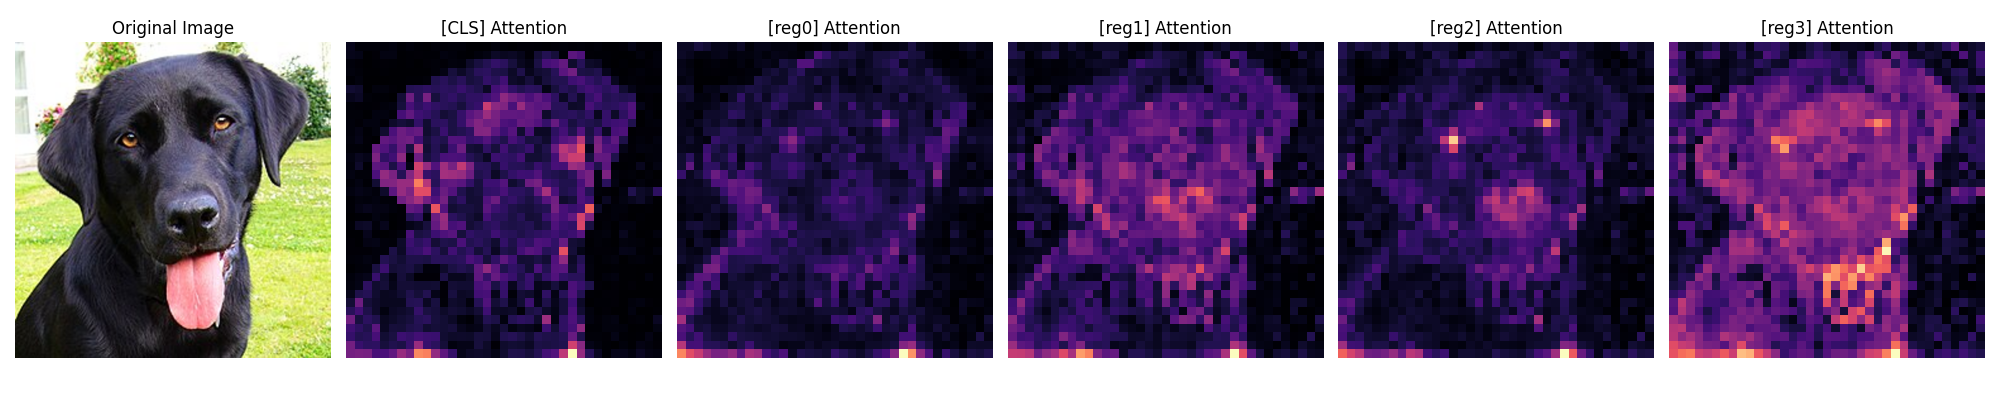
\includegraphics[width=\textwidth]{../../src/Raffaele/img/dino_attention_maps_comparison.png}
\caption{Comparison of attention maps for DINOv2 of the \texttt{[CLS]} and register tokens.}
\label{fig:qualitative_attention}
\end{figure}

\begin{figure}[H]
\centering
    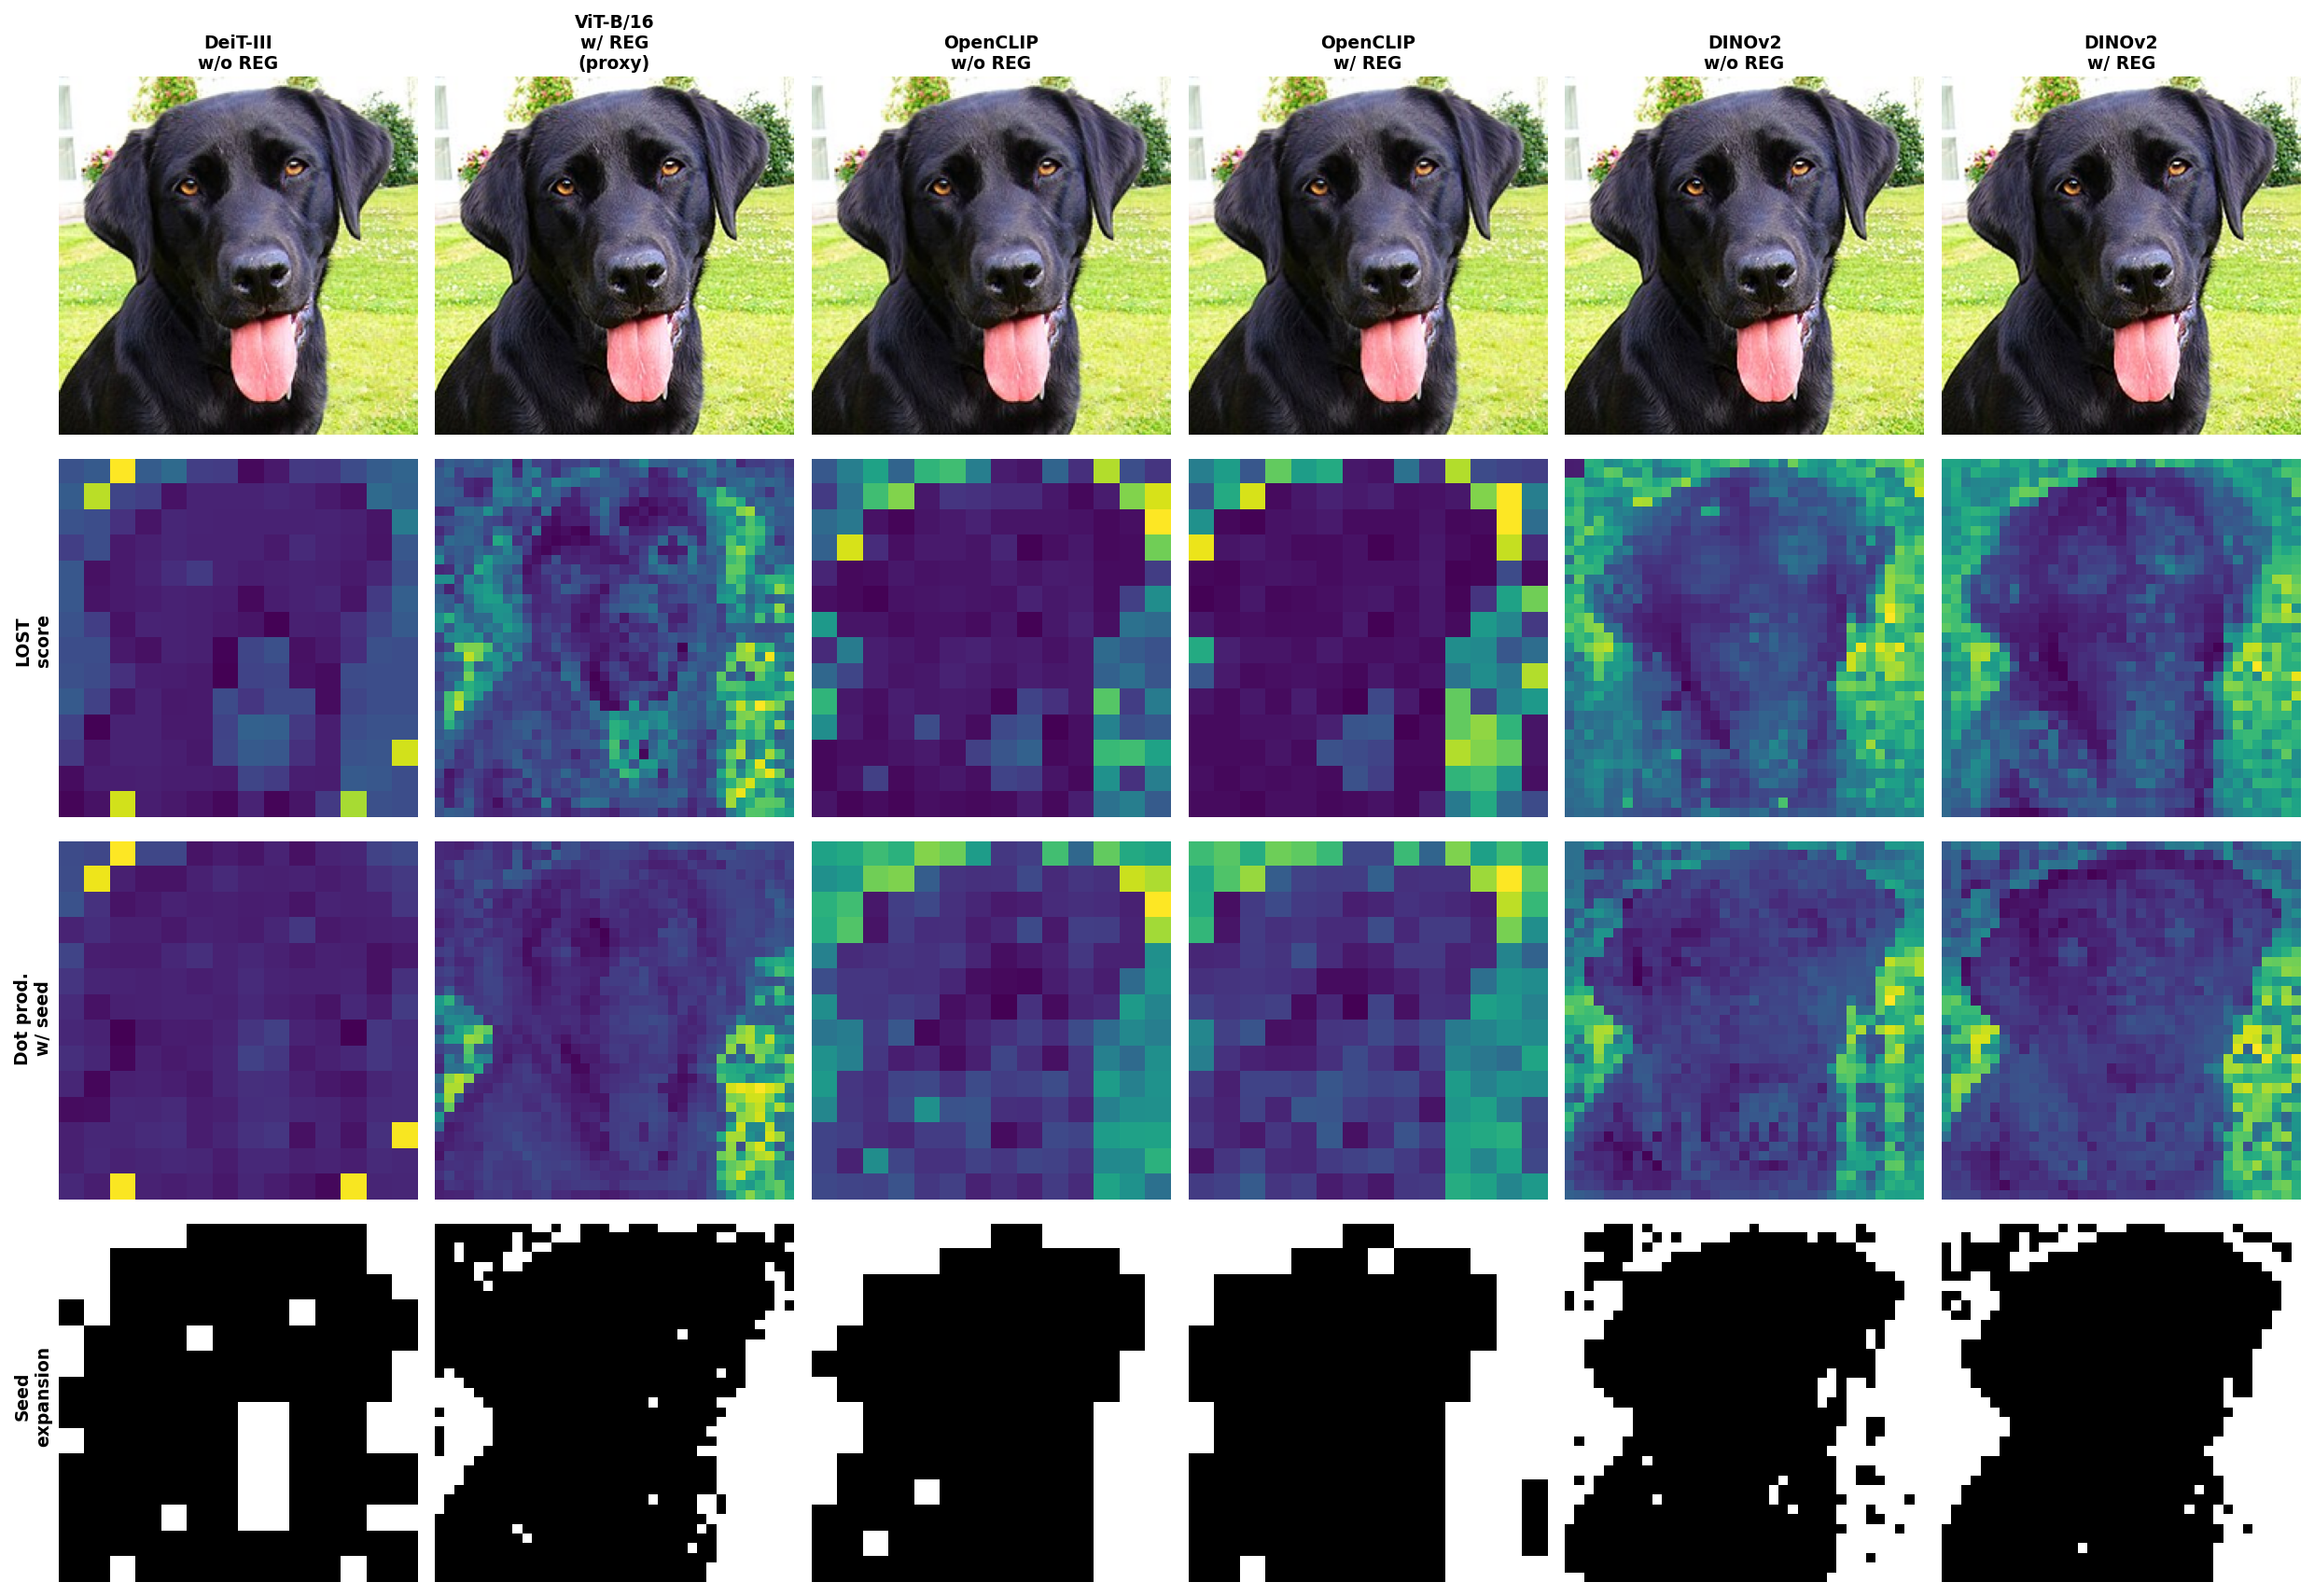
\includegraphics[width=0.8\textwidth]{../../src/Raffaele/img/figure_13_replication.png}
\caption{Intermediate computations in LOST algorithm for all models. Adding registers improves the look of intermediate steps.}
\label{fig:lost_intermediate_steps}
\end{figure}

\begin{figure}[H]
\centering
\begin{minipage}{0.65\textwidth}
    \centering
    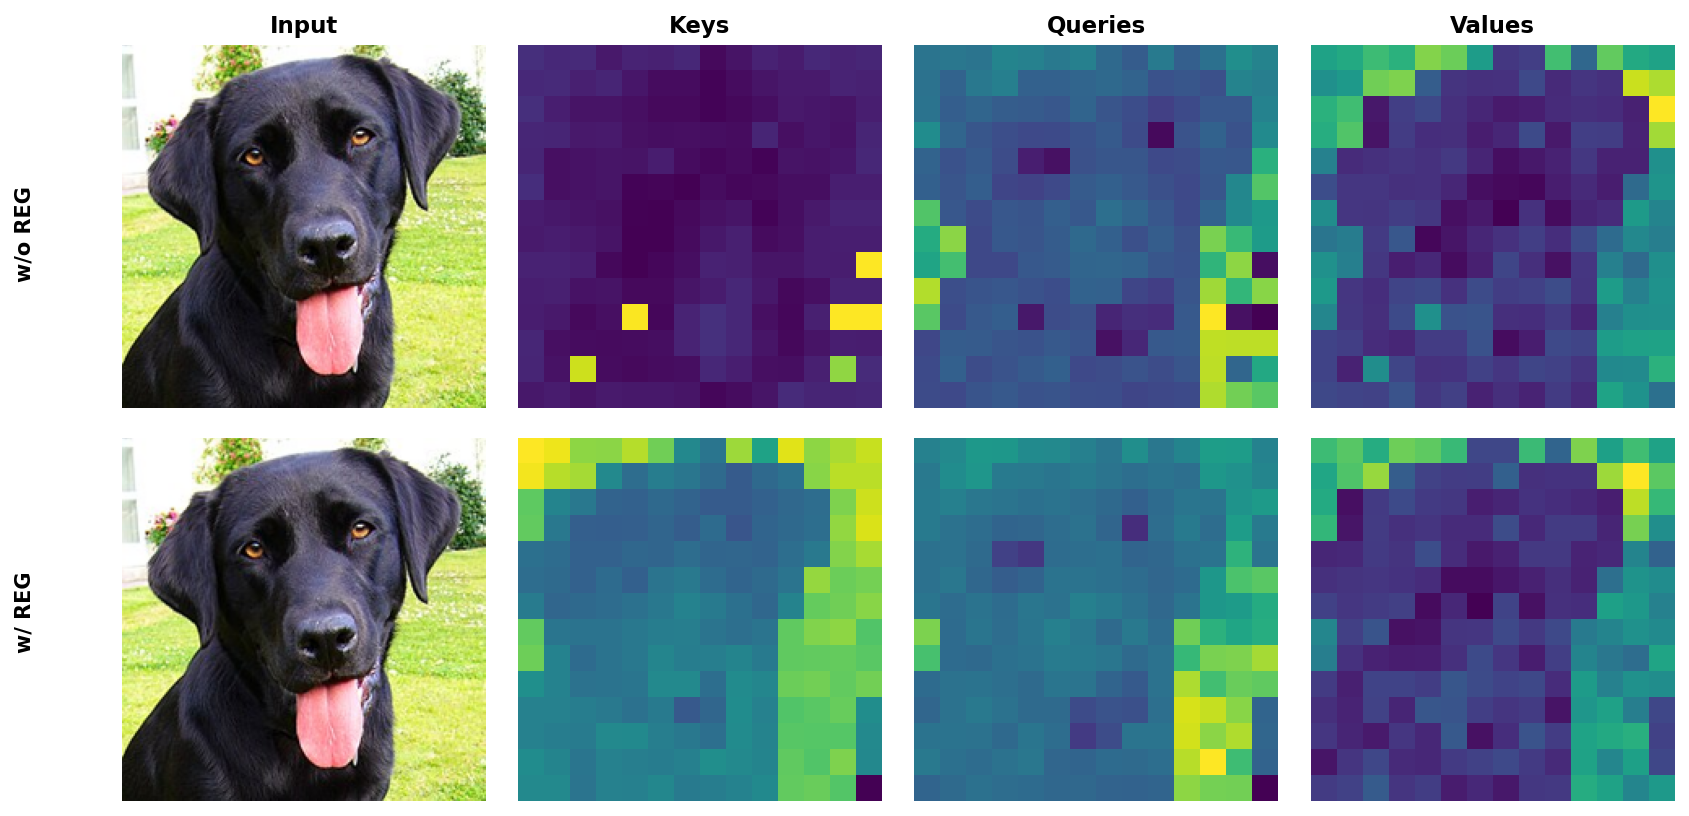
\includegraphics[width=\textwidth]{../../src/Raffaele/img/figure_14_replication.png}
    \caption{Seed expansion score in LOST for OpenCLIP with and without registers for keys, queries, and values.}
    \label{fig:seed_expansion_openclip}
\end{minipage}
\hfill
\begin{minipage}{0.3\textwidth}
    \centering
    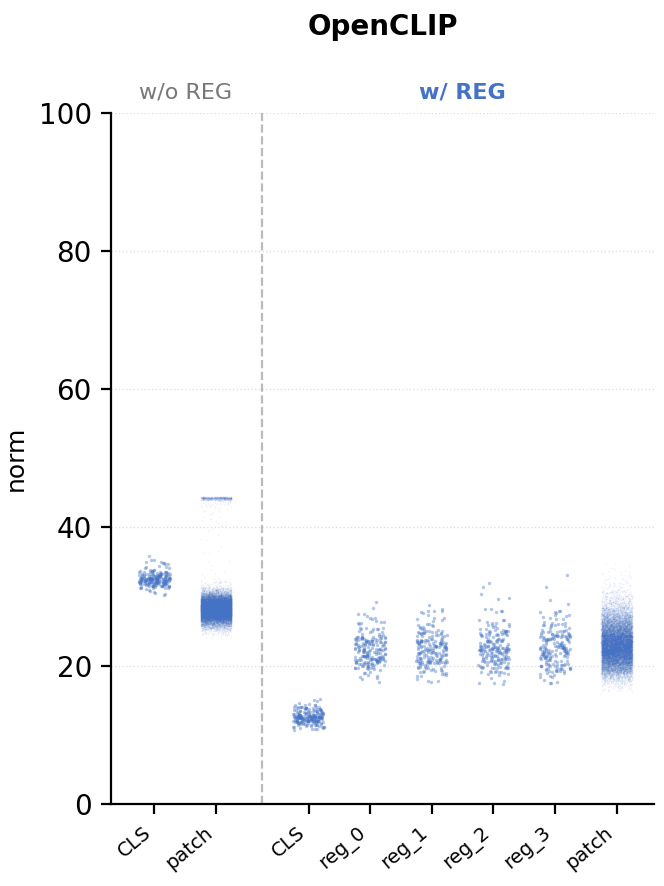
\includegraphics[width=\textwidth]{../../src/Raffaele/img/figure_7_OPENCLIP.png}
    \caption{Effect of registers on the distribution of token norms for OpenCLIP.}
    \label{fig:token_norms_openclip}
\end{minipage}
\end{figure}

\begin{figure}[H]
\centering
    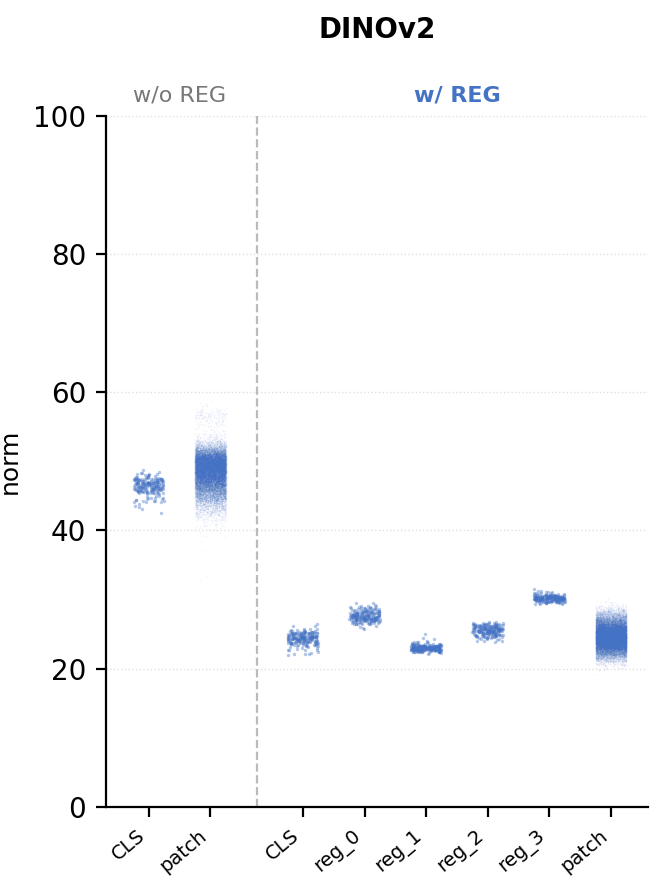
\includegraphics[width=0.3\textwidth]{../../src/Raffaele/img/figure_15_replication.png}
\caption{Distribution of token norms for DINOv2 with and without registers. Registers reduce the number of high-norm outlier tokens among patch tokens.}
\label{fig:token_norms_dinov2}
\end{figure}

\begin{table}[H]
\caption{Top-1 accuracy (\%) of linear probes of models with and without registers on FGVC-Aircraft dataset. Format shows accuracy for our replication / paper reference.}
\label{tab:outlier_token_probes}
\begin{center}
\resizebox{35em}{!}{%
\begin{tabular}{lcccc}
\toprule
\textbf{Model} & \textbf{[CLS]} & \textbf{Normal patch} & \textbf{Outlier patch} & \textbf{Register}\\
\midrule
DINOv2-giant w/o reg &  90.7 / 84.6 & 13.9 / 15.5 & 81.9 /73.3 & N/A / N/A \\
DINOv2-giant w/ 4 reg &  88.3 / 85.2 & 21.2 / 14.5 & N/A / N/A & 82.7 / 71.1 \\
\bottomrule
\end{tabular}
}
\end{center}
\end{table}

\begin{table}[H]
\caption{Local information probing results for DINOv2-giant with and without registers. Format shows accuracy for our replication / paper reference.}
\label{tab:local_information_probes}
\begin{center}
\resizebox{35em}{!}{%
\begin{tabular}{lccc}
\toprule
& & \multirow{2}{10em}{\textbf{Pos prediction top-1 accuracy}} & \multirow{2}{5em}{\textbf{Reconstruction L2 error $\downarrow$}}\\
\textbf{Model} & \textbf{Patches considered} &  & \\
\midrule
DINOv2-giant w/o reg &  non-outliers & 82.0 / 66.3 & 2.8 / 15.9 \\
DINOv2-giant w/ 4 reg &  non-outliers & 76.5 / 65.8 & 2.9 / 16.0 \\
\bottomrule
\end{tabular}
}
\end{center}
\end{table}

\begin{figure}[H]
\centering
    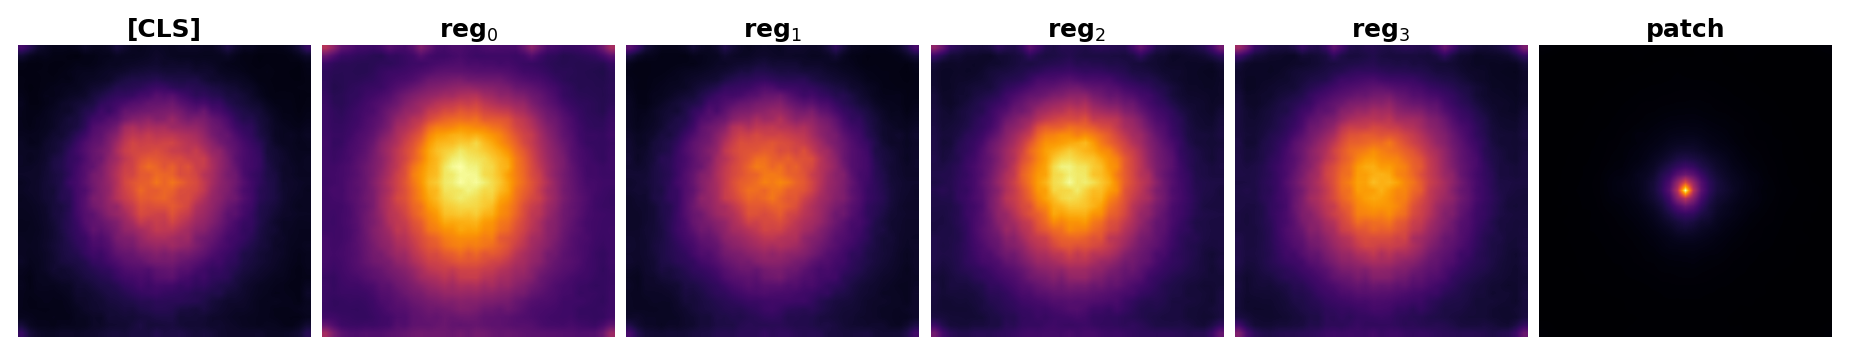
\includegraphics[width=0.8\textwidth]{../../src/Raffaele/img/figure_16_replication.png}
\caption{Positional focus of attention weights for DINOv2-giant with and without registers.}
\label{fig:positional_focus}
\end{figure}